\documentclass[a4]{scrreprt}
\usepackage[ngerman]{babel}
\usepackage[latin1]{inputenc}
\usepackage{graphicx}
\usepackage{<copytex:hhb/formulare/picins.sty>}
\usepackage{color}
\usepackage{wasysym}

\renewcommand{\familydefault}{\sfdefault} 
\usepackage{helvet} 
\usepackage[rotate]{crop}

\usepackage{<copytex:hhb/wallpaper.sty>}
\setlength{\headheight}{12\baselineskip}	% kleiner=h�her

\begin{document}
%IFINTERN
Das Transplantat Sp<var:IDSpender><var:SPAuge> wurde am  <var:EndeWarteliste> folgenderma"sen verwendet:\\

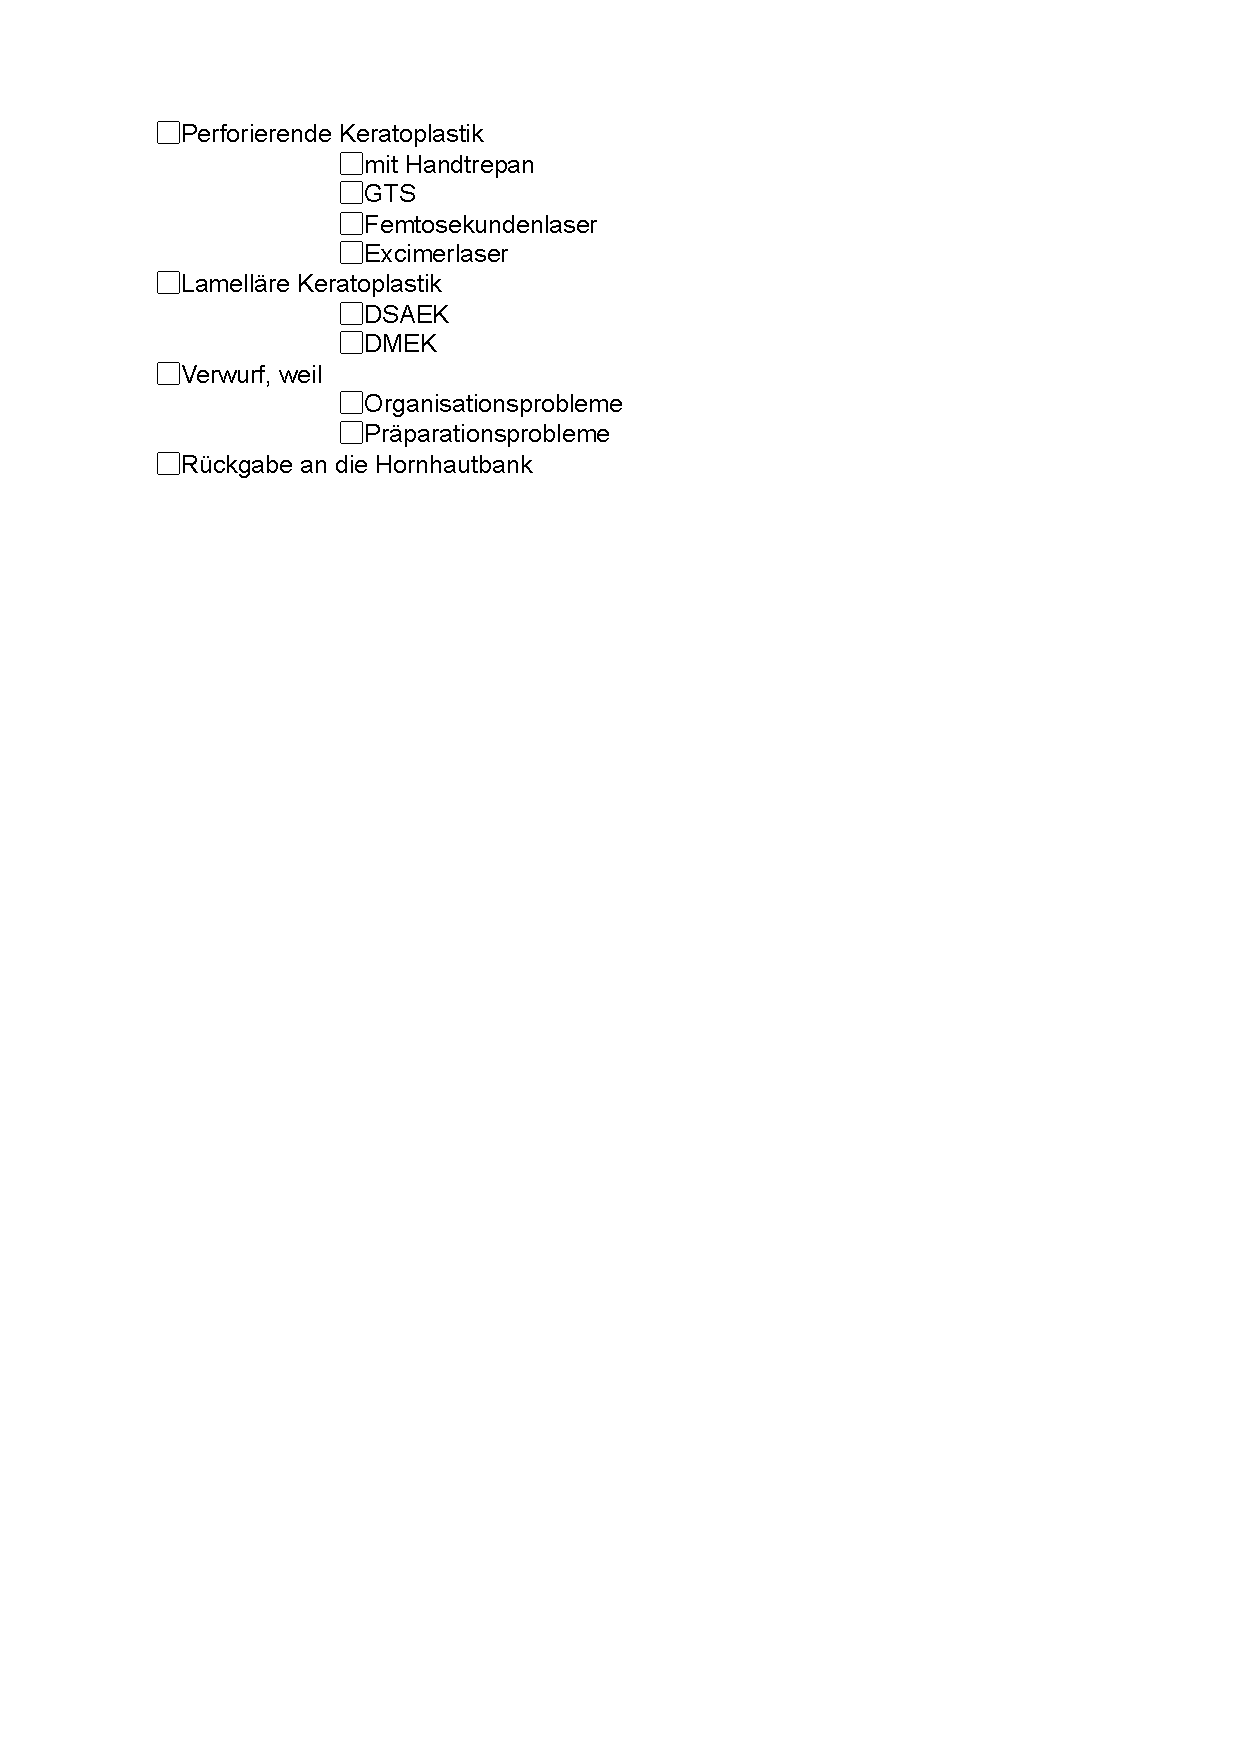
\includegraphics{<file:formulare/rueckseite_tp_bogen.pdf>}
%/IFINTERN

\begin{itemize}
\item Sie erhalten eine humane Hornhaut in Organkultur. Die Hornhaut hat unsere Hornhautbank in gutem Zustand und ohne Anzeichen einer Besch"adigung oder mikrobiellen Kontamination verlassen.
\item Die Hornhaut darf nicht verwendet werden, wenn die Transportdose besch"adigt ist, die Hornhaut nicht vom Medium bedeckt ist, das Medium nicht klar ist (Anzeichen einer mikrobiellen Kontamination).
\item Ist einer dieser Punkte nicht erf"ullt, ist vor Transplantation zwingend Kontakt mit der Hornhautbank aufzunehmen.Vor der Verwendung sind die Identit"at des Empf"angers und des Transplantates sicherzustellen.
\item Eine andere Verwendung als die angegebene ist nur nach R"ucksprache mit der Hornhautbank m"oglich.
\item Wir sind gesetzlich verpflichtet den Zustand des Transplantates bei Ankunft am Operationsort sowie  den fr"uhen postoperativen Verlauf zu dokumentieren. Bitte faxen Sie daher den beigef"ugten Qualit"atsicherungsbogen an folgende Nummer: +49 761-270-41310. Sollten wir wiederholt keine ausgef"ullten Qualit"atssicherungsb"ogen erhalten, k"onnen wir keine Transplantate mehr abgeben.
\item Sollten Sie w"ahrend oder nach der Transplantation eine schwerwiegende unerw"unschte Reaktion feststellen, die mit der Qualit"at  des Transplantates in Zusammenhang stehen k"onnte, bitten wir um umgehende R"uckmeldung mit dem beigelegten Formular zun"achst an die Faxnummer +49 761-xx. Die Hornhautbank "ubernimmt die Weiterleitung an das Paul-Ehrlich-Institut.

\end{itemize}
\newpage
\setlength{\oddsidemargin}{-18mm} 
\addtolength{\textwidth}{1cm}

\ThisCenterWallPaper{1}{<file:briefkopfHHB2.pdf>}
\subsubsection{~~~~~~Humane Augenhornhaut, organkultiviert, Freiburg f"ur Transplantation}
{\parpic(8cm,10cm)(2cm,10.2cm)[r]{\includegraphics[width=7.5cm]{<var:endothelpath>}}}
\begin{tabular}{lp{10.3cm}l} \hline
Transplantatnummer & Sp<var:IDSpender><var:SPAuge>\\
Spenderalter & <var:SpenderAlter> (<var:Spendergenus>)\\
HIV-Serologie & negativ\\
HCV-Serologie / RNA-PCR & negativ\\
HBs-Ag & negativ\\
TPPA & negativ\\
Tod-Entnahme-Zeit (Stunden)  & <var:PostMortemZeit>\\
Kulturdauer gesamt (Tage) & <var:KulturdauerGesamt> \\
Kulturdauer Medium 2 (Tage) & <var:KulturdauerAktuell> \\
Letzte mikroskopische Kontrolle & <var:DatumLetzteEZD> \\
Freigegeben durch Arzt & <var:PersonKontrolle> \\
Endothelzelldichte & <var:LetzteEZD> ${Zellen \over mm^{2} }$ \\
Letzte mikrobiologische Kontrolle & <var:DatumLetzteMiBi> (steril) \\
\\ \hline
Empf"anger & <var:Name>, <var:Vorname>, geb. am <var:Geburtsdatum>\\
Operationsdatum & <var:EndeWarteliste>\\ 
Verwendbar bis  & <var:HaltbarBis>\\
Auge & <var:OPAuge>\\ 
Verwendungszweck & <var:Verwendungszweck>~{\bf {\large\Square} best"atigt {\large\Square} andere OP \RIGHTarrow  wenden} \\ 
Indikation & <var:OPDiagnose>\\ 
Zentrum & <var:Zentrum>\\ 
\hline
HLA Splits Spender & <var:HLASpender>\\
HLA Splits Patient & <var:HLAPatient>\\
\hline
Bemerkung & <var:OKBemerkungen> 
\\ \hline
\\
\end{tabular}

\begin{tabular}{p{16.5cm}}
Die Kennzeichnung und die Freigabe des Gewebes entsprechen den Vorgaben des Qualit"ats\-managementhandbuches bzw. der Genehmigungsunterlagen.\\ \\
\end{tabular}

\begin{tabular}{p{2cm}p{3.2cm}l}
<var:Datum> & Unterschrift  & Dr. Philip Maier
\\
&& {\small Verantwortliche Person nach �20c des Arzneimittelgesetzes}\\
\end{tabular}

\fcolorbox{red}{white}{\parbox{1.05\textwidth}{
\tiny
{ \bf Vor der Operation muss das Gewebe zur Beseitigung von Kulturmediumr"uckst"anden in steriler isotonischer Kochsalzl"osung geschwenkt werden.

Vor der Operation unbedingt die Transplantatnummer auf der beiliegenden Flasche mit der Nummer auf diesem Transplantatbogen abgleichen.

Bei Raumtemperatur, aufrecht lagern! Nicht k"uhlen, nicht einfrieren, nicht bestrahlen!}

Das Transportmedium enth"alt Penicillin, Streptomycin, Dextran 500 und Amphothericin B sowie 2\% Newborn Calf Serum.

Entsprechende allergische Dispositionen des Empf�ngers sind zu beachten.

}}


\bf{\scriptsize  ~

Gen-Nr.: PEI.G.1xx\\}
\bf{ Wichtige Hinweise: siehe R"uckseite}

\end{document}
